%
% File acl2014.tex
%
% Contact: giovanni.colavizza@epfl.ch
%%
%% Based on the style files for ACL-2013, which were, in turn,
%% Based on the style files for ACL-2012, which were, in turn,
%% based on the style files for ACL-2011, which were, in turn, 
%% based on the style files for ACL-2010, which were, in turn, 
%% based on the style files for ACL-IJCNLP-2009, which were, in turn,
%% based on the style files for EACL-2009 and IJCNLP-2008...

%% Based on the style files for EACL 2006 by 
%%e.agirre@ehu.es or Sergi.Balari@uab.es
%% and that of ACL 08 by Joakim Nivre and Noah Smith

\documentclass[11pt]{article}
\usepackage{acl2014}
\usepackage{times}
\usepackage{url}
\usepackage[hidelinks]{hyperref}
\usepackage{latexsym}
\usepackage{graphicx}
\usepackage{caption}

%\setlength\titlebox{5cm}

% You can expand the titlebox if you need extra space
% to show all the authors. Please do not make the titlebox
% smaller than 5cm (the original size); we will check this
% in the camera-ready version and ask you to change it back.

% !TeX spellcheck = en_GB 

\title{Of Recipes and Ingredients}

\author{Redouane Elghazi \\
  {\tt redouane.elghazi@epfl.ch} \\\And
  \\\\\textbf{Pierre Mahmoud--Lamy} \\
  {\tt pierre.mahmoud-lamy@epfl.ch} \\\And
Enguerrand Prebet \\
{\tt enguerrand.prebet@epfl.ch} \\}

\date{}

\begin{document}
\maketitle
\begin{abstract}
	
	Can recipes be grouped into meaningful classes in terms of ingredients? Are these groups characterized by their distributions in carbs,fat and proteins?
\end{abstract}

\section{Database Presentation}
% - recipes with nutriments
We gathered the data from \newcite{WestWhiteHorvitzWWW2013}. This data contains recipes from several cooking websites. A recipe entry has informations such as the calories (fat, proteins, carb) and the list of the ingredients. 

% - external ingredients
To only extract the ingredients from the list, we used an external data base from \href{http://openfood.schoolofdata.ch}{openfood.schoolofdata.ch} as a starting point. It contains a list ingredients but also a groups for these ingredients such as "vegetables" or "cereals".

% - additional items added
We had to append words that were not in the database but that appear in recipes, especially for cheese names, pasta names and sauce names.

\section{Preprocessing the database}
% - extract ingredients list
Each recipe was represented as one long string. To only extract ingredients as opposed to quantities and others words that may appear in a recipe, we considered our external database with words sorted by decreasing length. For each ingredient, we then processed through the recipes and checked if it appeared in the string of ingredients. In that case, we added it to our list of ingredients and deleted it from the string.

By sorting and deleting ingredients, we ensure that combination of words like "black pepper" is found without also finding "pepper". Some words were still matched incorrectly, with "tea" found in recipes because of the use of "teaspoon", and "gin" found in "virgin" for instance. So before looking for our ingredients, we preprocessed the recipe by removing those words first.
We also took into consideration plural and separators.

% - normalize kcal
When looking at the nutritional informations, we saw that some recipes are too energetic to be normalized per serving, being over the recommended amount for one person \textbf{per day}. To be able to compare different recipes, we normalized our data by the total energy for the recipe, and thus considered proportion of fat, carb and proteins instead of their raw value.

\section{Clustering}
% - vector representation
To reorganize our different recipes into groups according to their ingredients, we need a decent representation. Our choice was to consider boolean value for each food group if a recipe contains an ingredients from that food group. This gives us a $N$-dimensional vector with value in $\{0,1\}^{N}$, with $N$ being the number of food group (11 in our case).

% - k-means(full copy-paste + 11->N)
We use a K-means clustering algorithm to create our recipe groups. Starting from K random means, we assign each recipe to the closest mean (the distance being defined as the sum of differences over the $N$ elements). Then each mean is updated to correspond to the effective mean of the elements assigned to this mean.

In practice, though recipes get values in $\{0,1\}^{N}$, the means have real values in $[0,1]^{N}$ to get the best possible clustering.

Moreover, after having tested different values of K to study the convergence of the groups, we set the option to fix the initial means, for reproducibility.

\section{First results}
%- results (full pompé)
After several tests, the more meaningful number of groups seems to be 4. By meaningful, we mean that we can visualize what the groups represent. Recall that the output of the algorithm is the assignement vector for each recipe, and the mean vectors. We then need to interpret the meaning of those means:

\begin{itemize}
\item the first group represents desserts based on complex preparations, mostly with eggs and flour or other cereal base, such as pies, cakes, muffins,...
\item the second group represents more simple desserts, with fewer ingredients and more fruit-based, such as fruit salads, baked apples,... but also chocolate mousse,...
\item the third group consists in complex prepared meals, with meat and vegetables. It uses a lot of different food groups (eggs, dairy, fats) and can for example be stews, boeuf bourguignon,...
\item the last group is easy-to-do dishes with meat and vegetables. It uses more condiments (mustard, sauces,...) and can be bolognese pasta, hot-dogs,...
\end{itemize}

The split of the groups can be considered using 2 questions:
\begin{itemize}
	\item Is this a main course ?
	\item Is it simple ?
\end{itemize}

\section{Classification by the nutrients}
% - analysis of distributions (je ne sais pas trop quoi dire à part redire la même chose mais sans les graphes c'est, chô)

\begin{figure}[!h]
	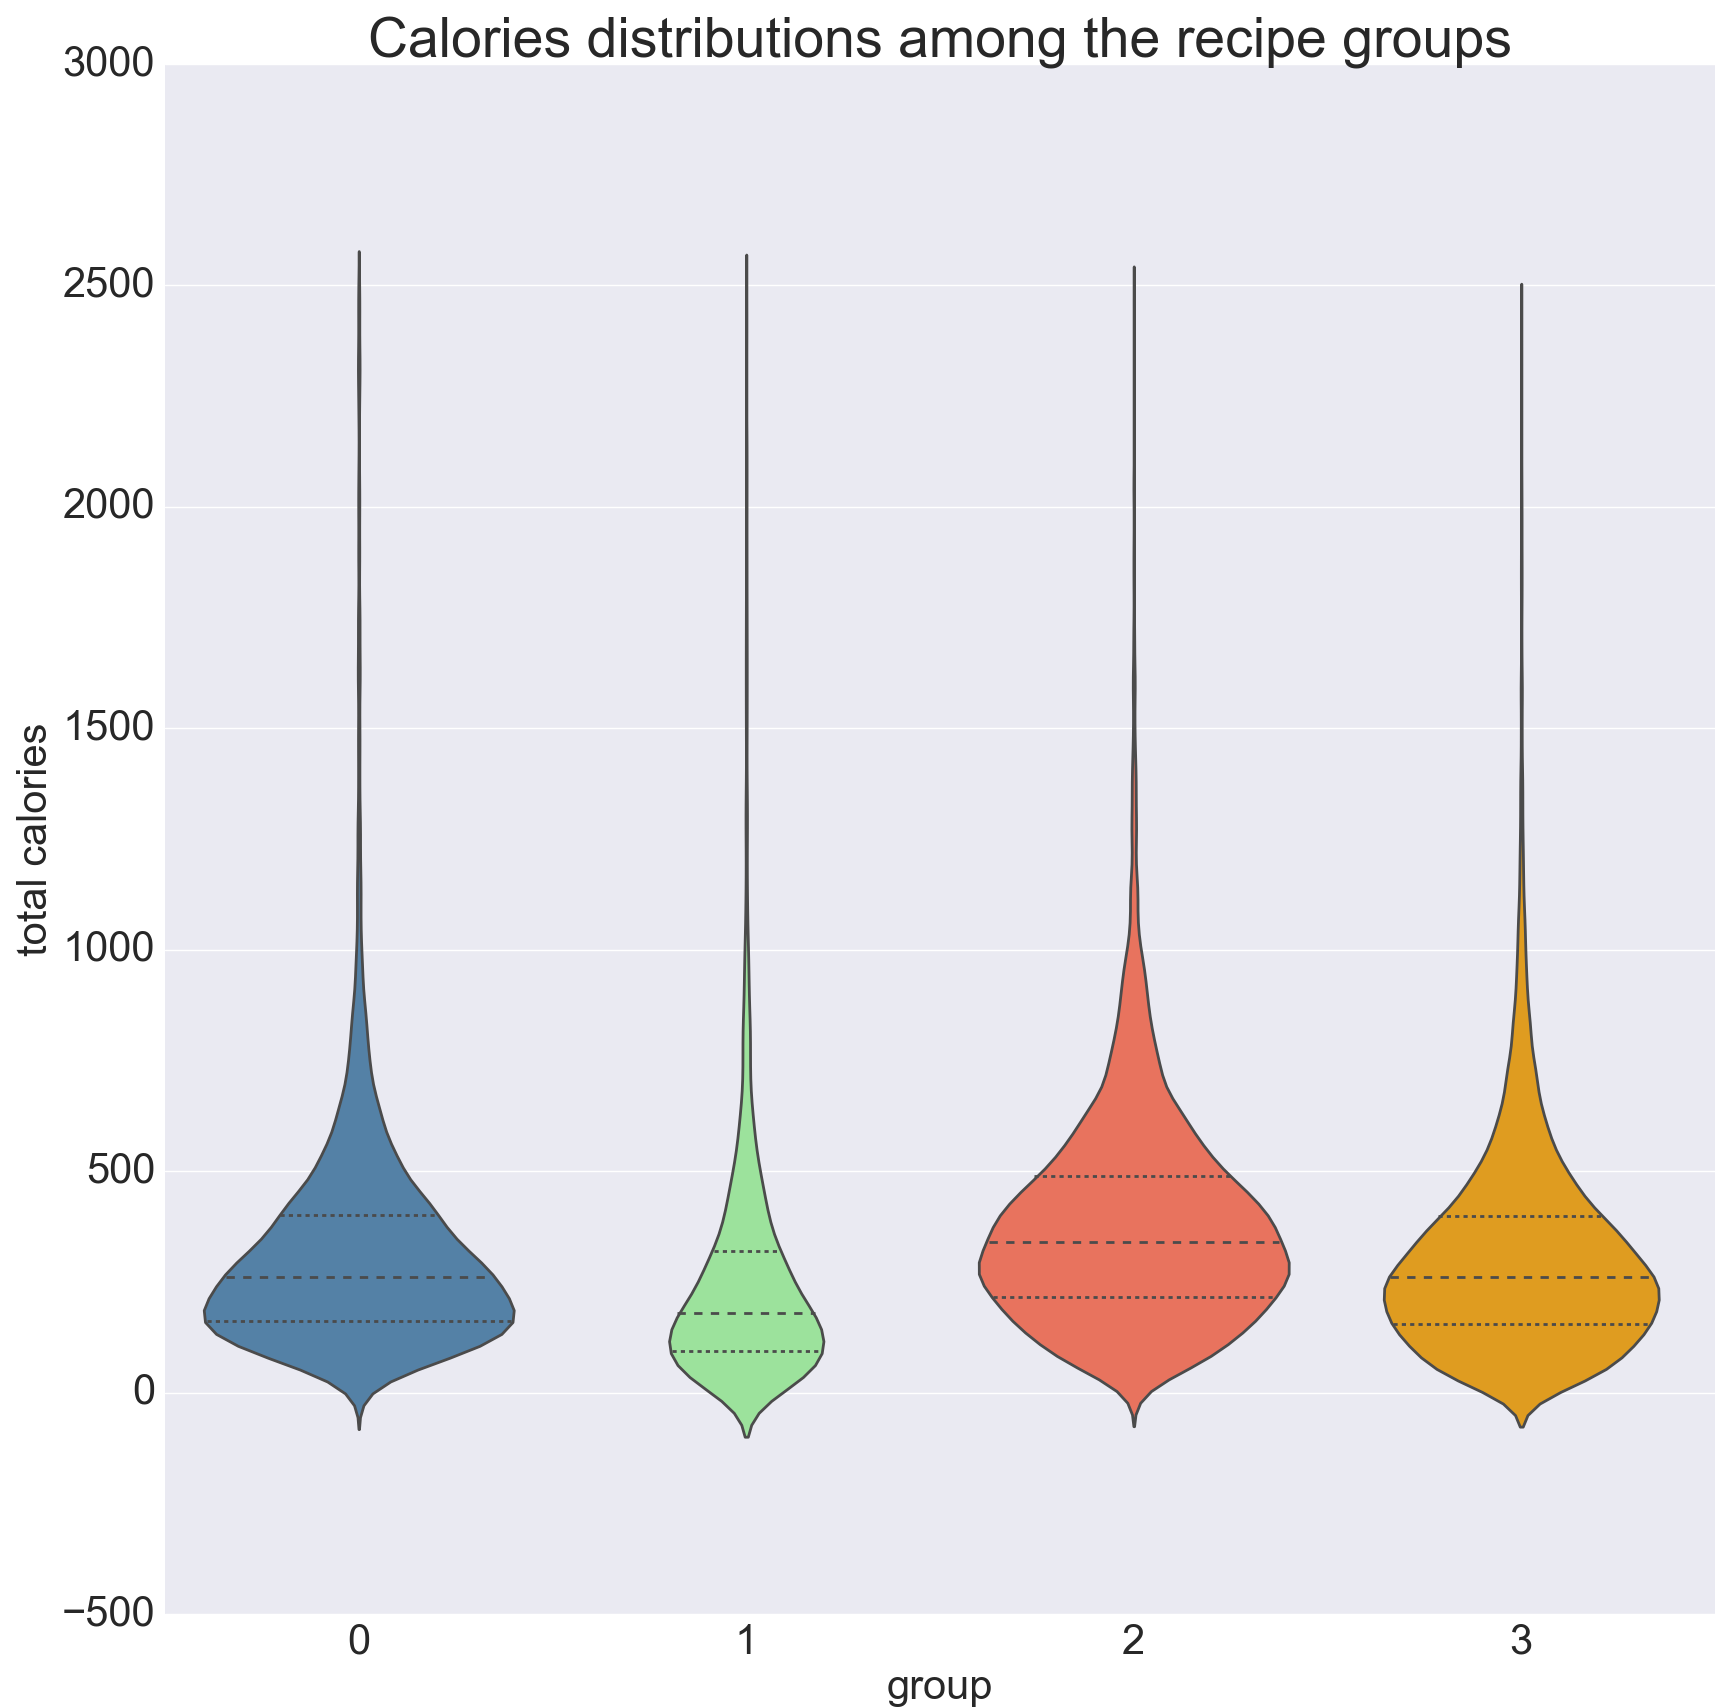
\includegraphics[width=\columnwidth]{../total_kcal_distrib-r.png}
	\caption{}
	\label{fig:1}
\end{figure}

We see that more complex recipes (0,2) have more calories than their simpler counterparts (respectively 1,3).

Moreover, quite surprisingly, main courses recipes (2,3) are in average more calorific than dessert recipes (0,1). They also have more recipes with very high calories, compared to dessert recipes.

This could be linked to desserts often considered full of fats and sugar, thus pushing people to develop and publish a lot of low-fat, low-calories dessert recipes in the 2010's. It also comes with the fact that there are a lot of subtitutes for sugar, milk and eggs.

\begin{figure}[!h]
	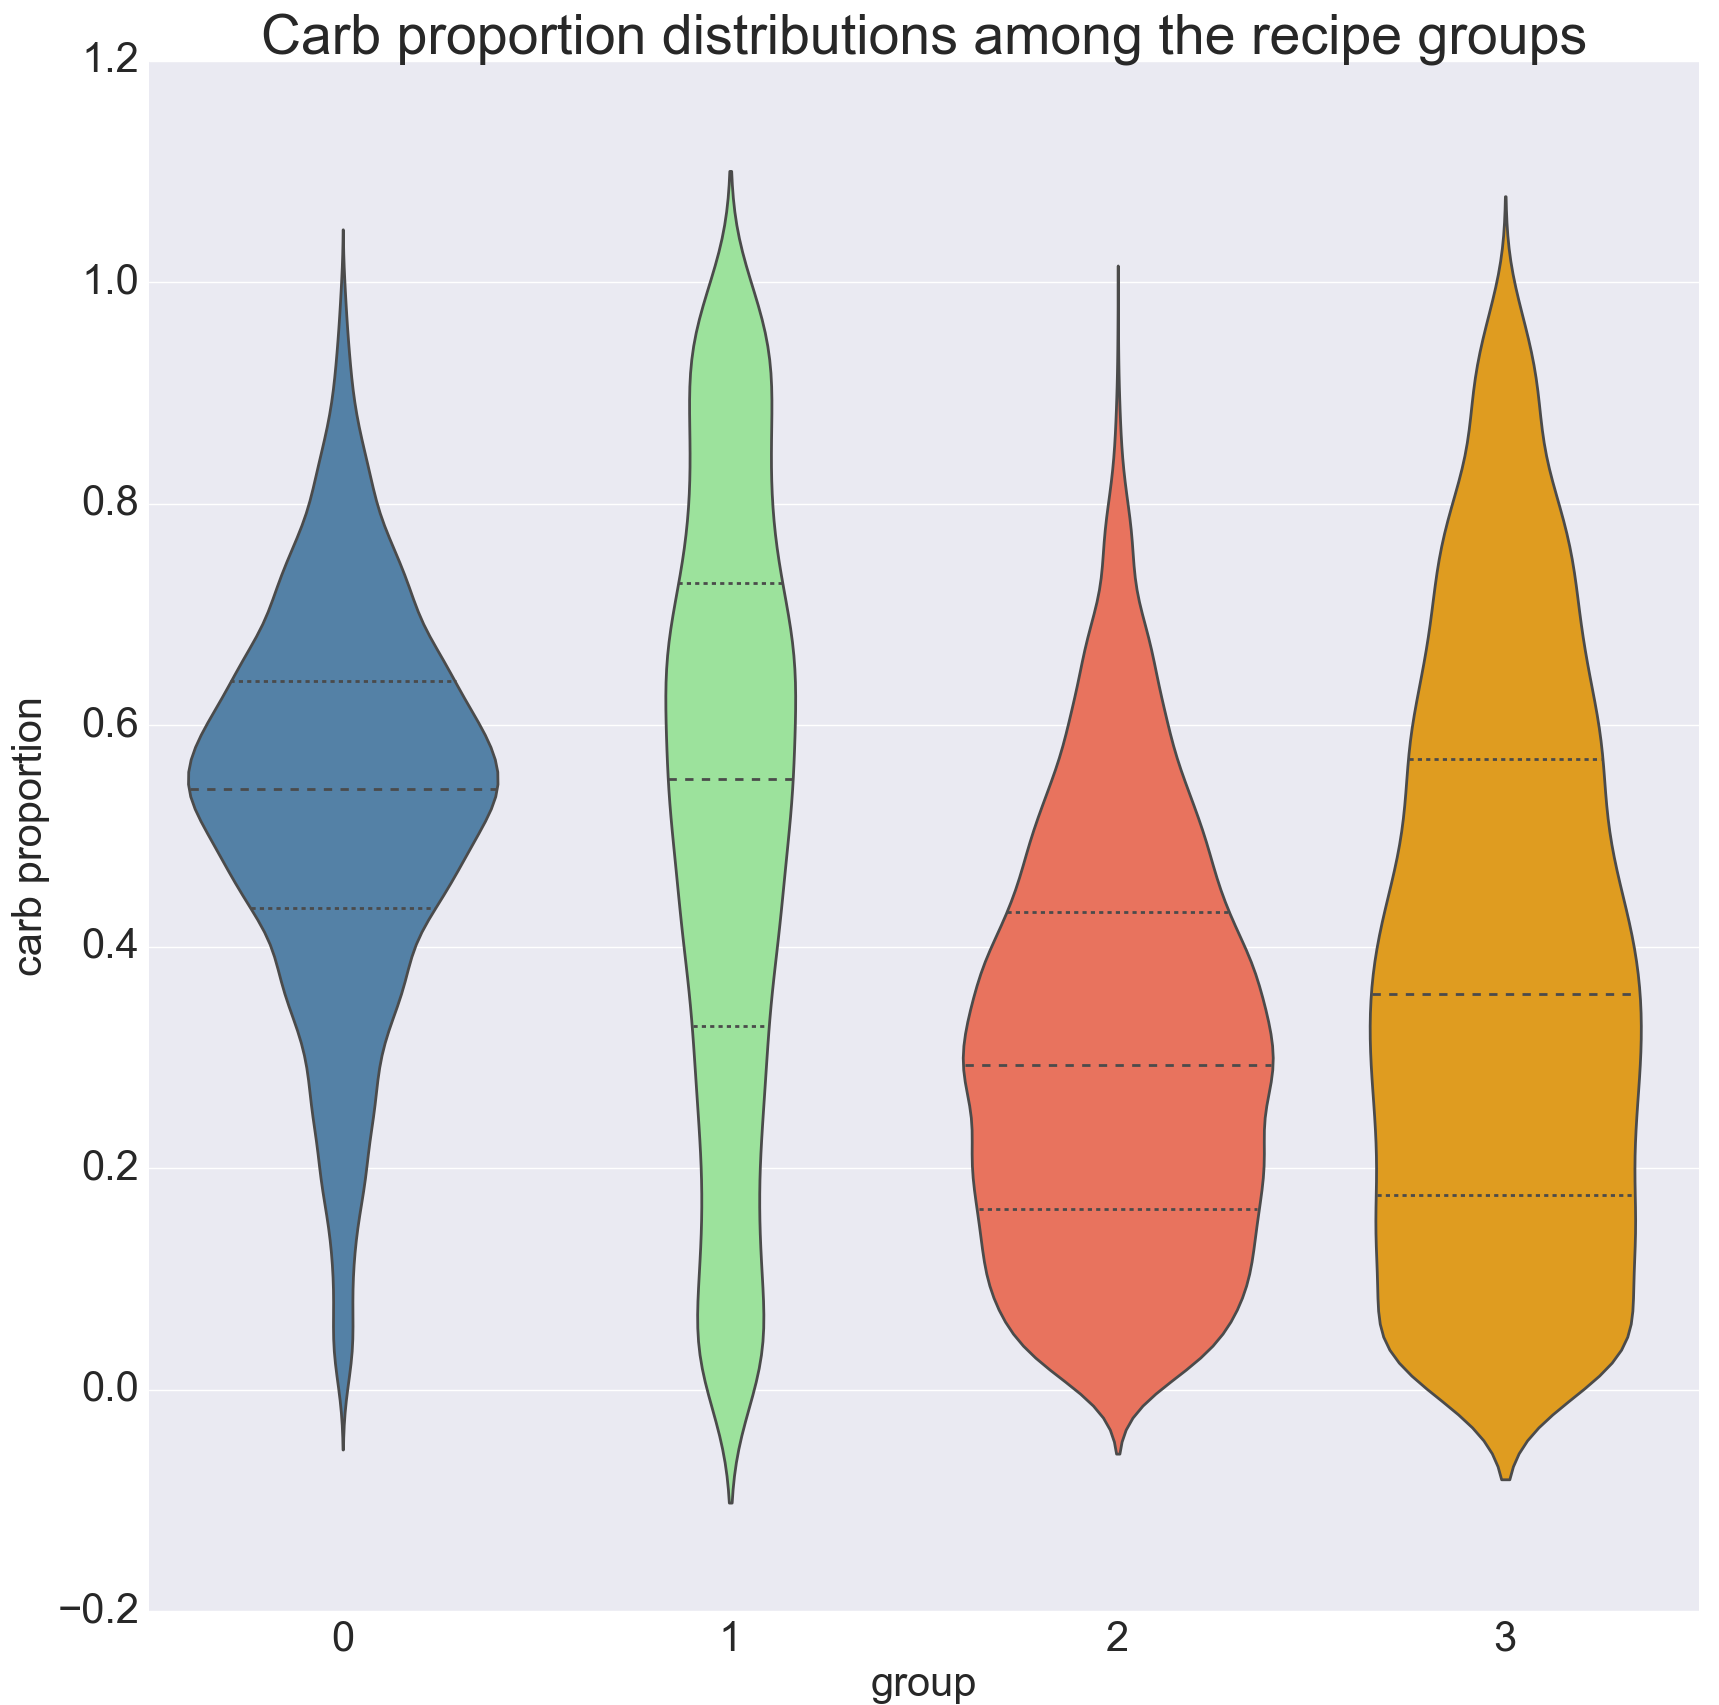
\includegraphics[width=\columnwidth]{../carb_prop_distrib-r.png}
	\caption{}
	\label{fig:2}
\end{figure}

We observe very different distributions of the carb proportion:

group 0 is pretty gathered around its mean, which is quite high. It seems complex desserts have high rates of carbs.
group 1 is quite regular: there is almost a uniform distribution of carb proportions. Thus simple desserts are not characterized by their carb rate.
group 2 and 3 have pretty low carb rates compared to the desserts groups. However simple main courses (3) can get to a high rate of carbs.

\begin{figure}[!h]
	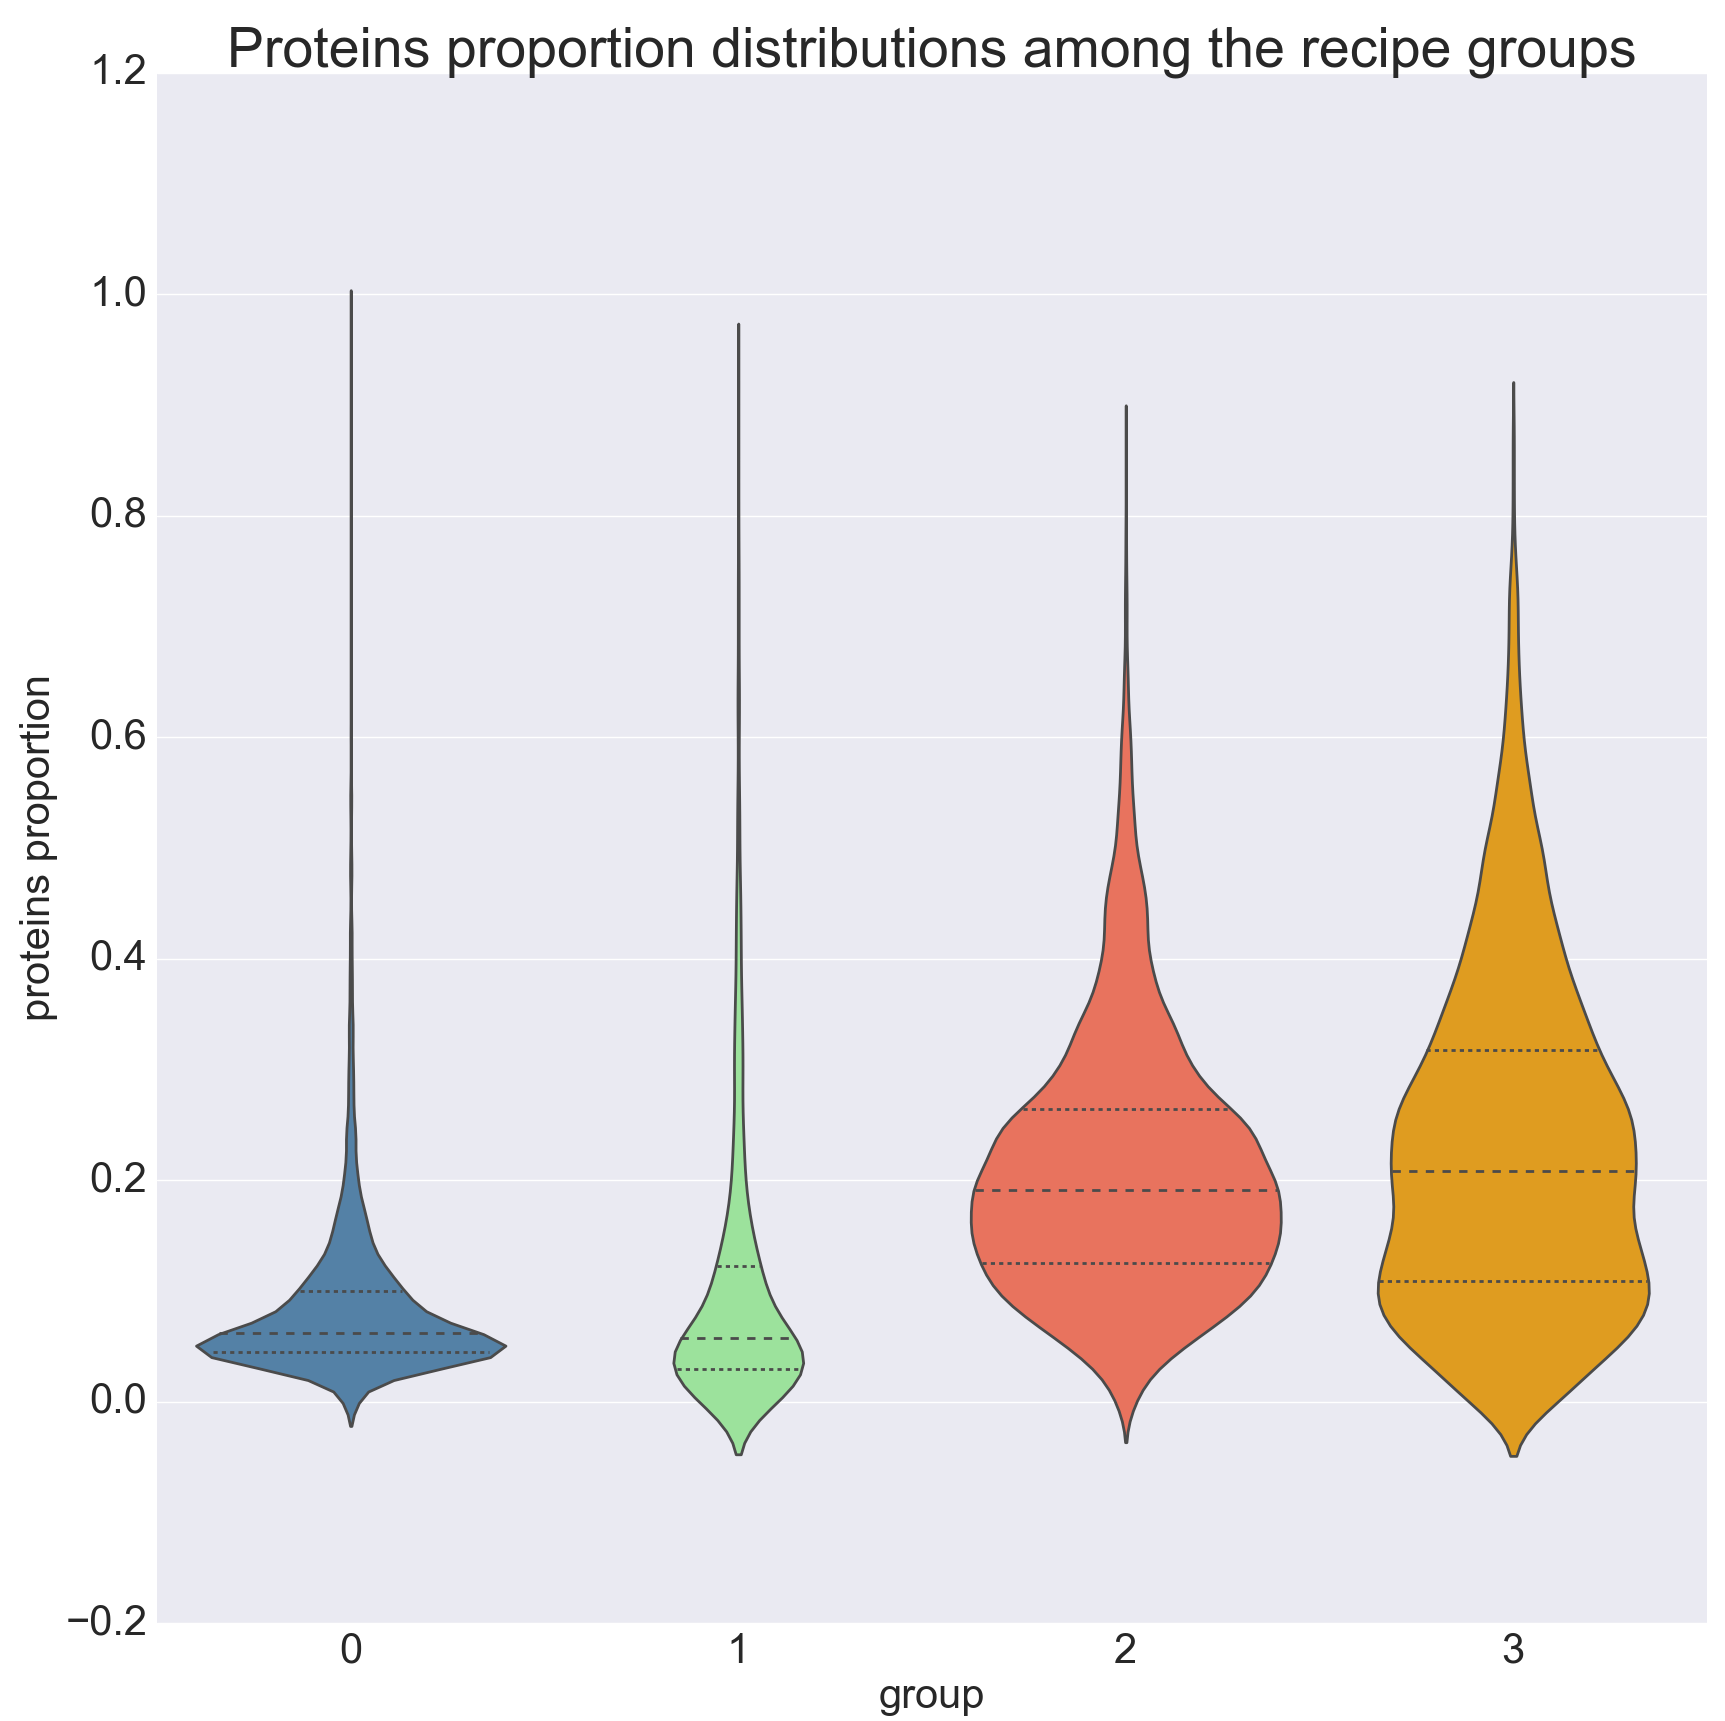
\includegraphics[width=\columnwidth]{../protein_prop_distrib-r.png}
	\caption{}
	\label{fig:3}
\end{figure}

For the proteins distribution, we can observe a great distinction between the desserts (0,1) and the main courses (2,3). The desserts have very low rates of proteins, and very centered around the mean.

The proteins proportion is sparse for the 2nd group, and even more spread for the 3rd group.

\begin{figure}[!h]
	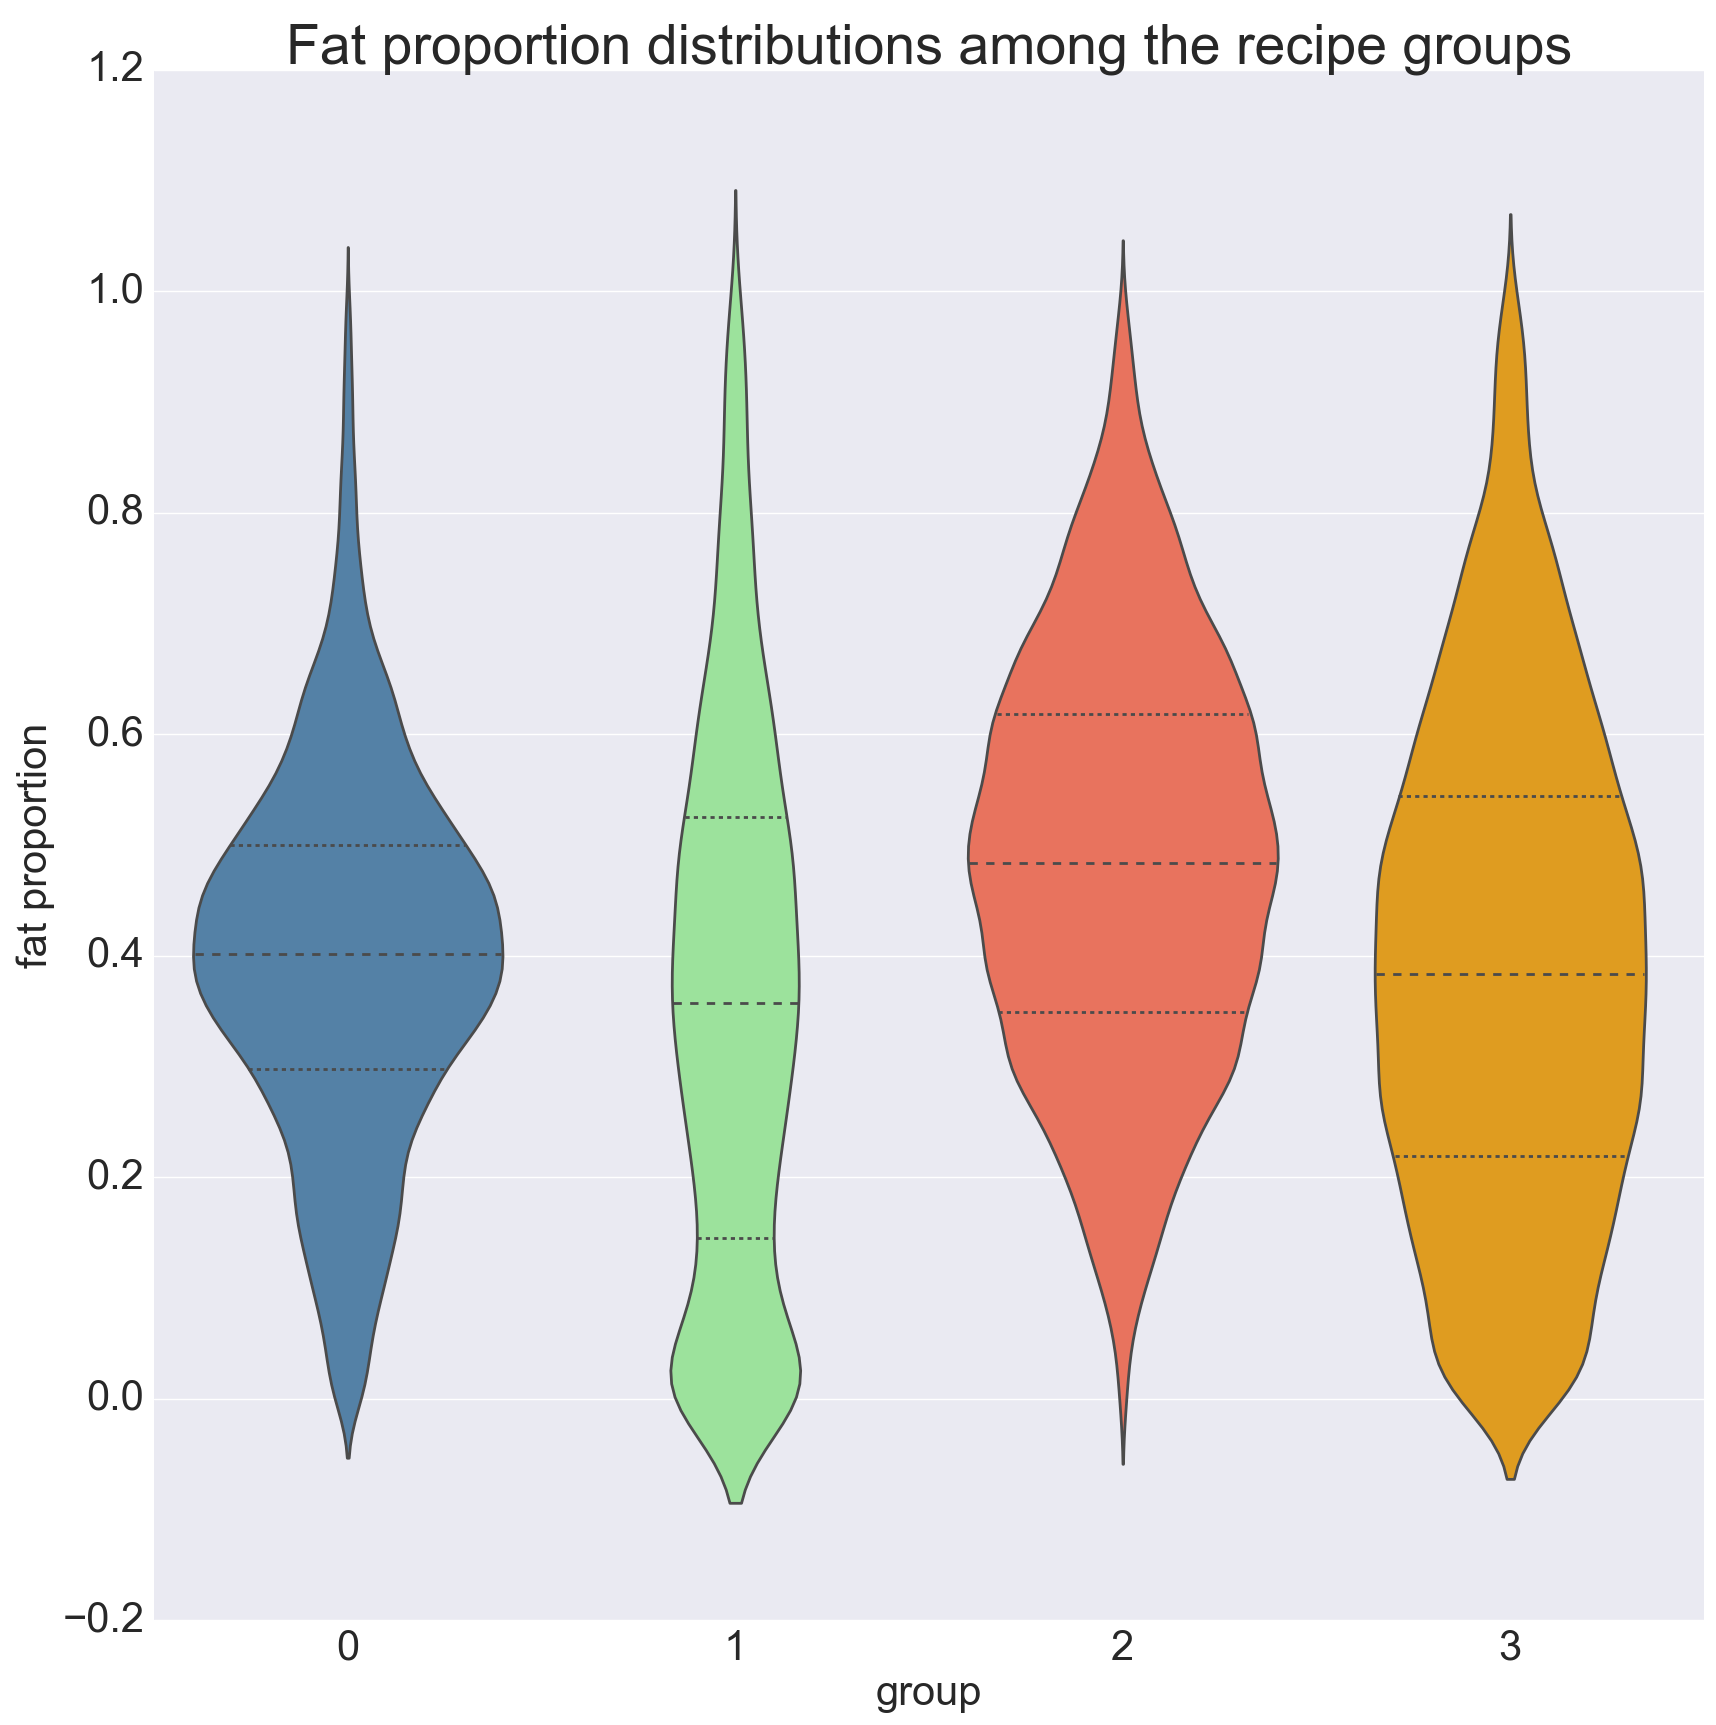
\includegraphics[width=\columnwidth]{../fat_prop_distrib-r.png}
	\caption{}
	\label{fig:4}
\end{figure}

The fat proportions are quite different among groups too. For group 1, the distribution is relatively uniform, a bit "squeezed" aroun the first quartile.

The distribution for group 0 is symmetric around the mean at 0.4, whereas distributions for groups 2,3 are more spread.

We also observe that complex recipes (0,2) have in average a higher fat rate than more simpler recipes (1,3).


% - propensity score
To test how well the nutrients describe the four groups, we use logistic regressions to obtain propensity scores for our 2 questions.

Our results are shown in \textsc{Figure} \ref{fig:end}. We notice mainly two things:
\begin{itemize}
\item the distinction main course/ dessert is pretty clear: groups 0 and 1 are both clearly identified as desserts. For groups 2 and 3, there is a residual tail but the main part is identified as main course
\item however the distinction between simple and complex recipes is not as correct. We see recipes are mostly considered simple, even if group 3 is not that far of being identified. Group 1 is quite out of the target zone.
\end{itemize}
\begin{figure*}
	\captionsetup{justification=raggedright,singlelinecheck=false}
	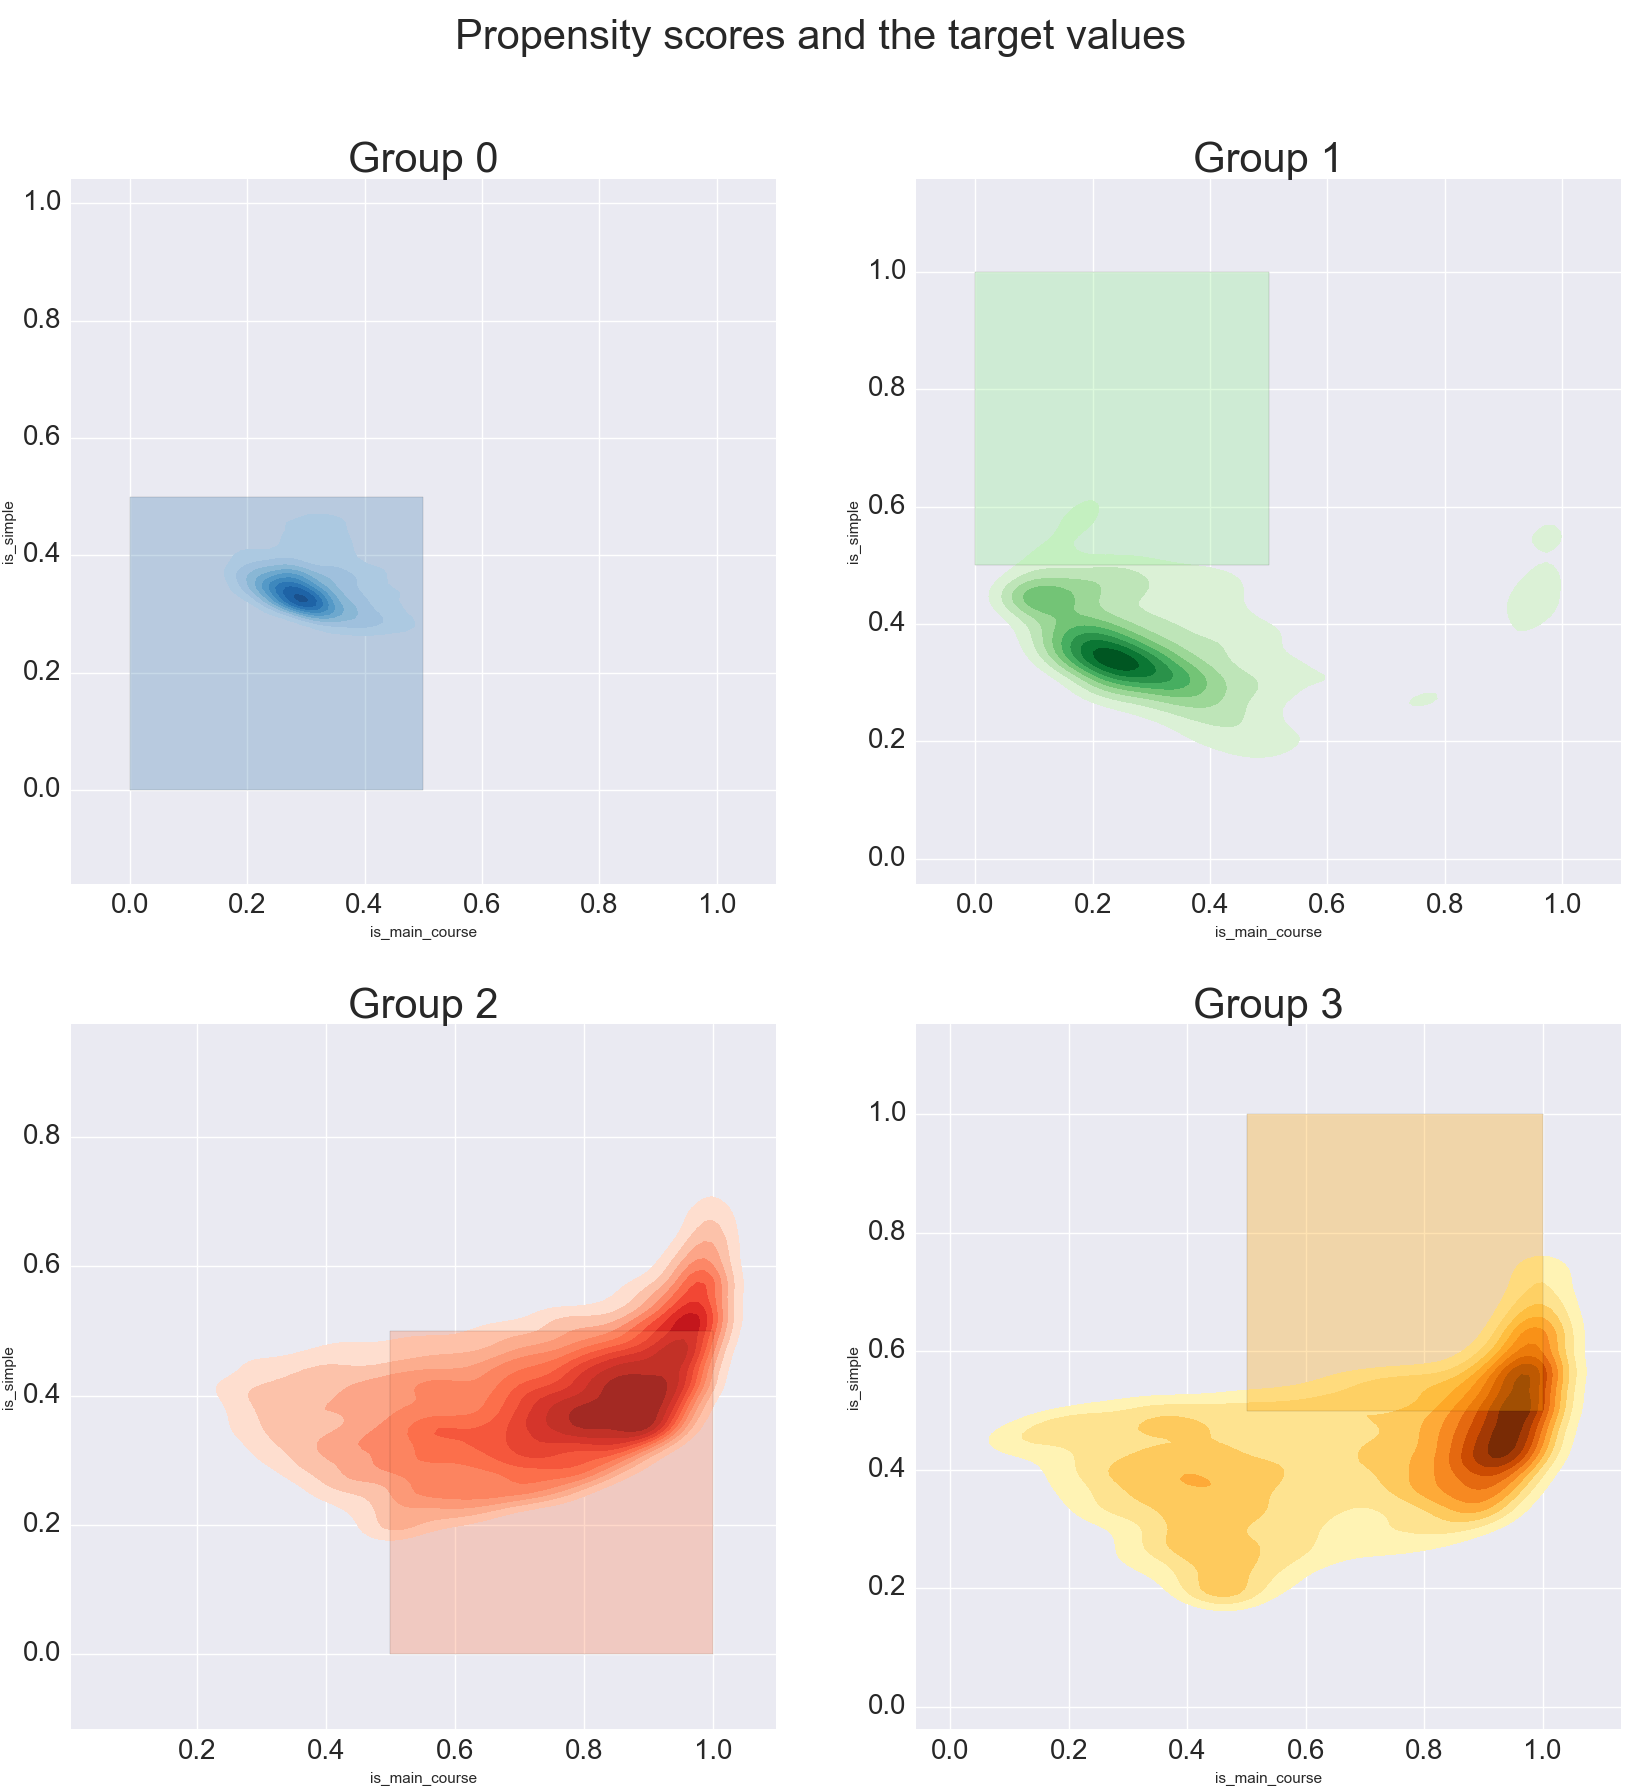
\includegraphics[width=\textwidth]{../propensity-r.png}
	\caption{}
	\label{fig:end}
\end{figure*}
\section{Conclusions}
From our analysis, we can answer our original questions. It clearly appeared that the recipes could be grouped into meaningful classes just using their ingredients. As for the characterization of these classes regarding their distributions in carbs, fat, and protein, the results are less sharp: among the 4 classes that we could create, only 2 seem to be discriminated. More precisely, we cannot distinguish a simple recipe from a complex one by just looking at the proportion of carbs, fat, and protein. Still we managed to distinguish desserts from main courses.

\begin{thebibliography}{}
	
	\bibitem[\protect\citename{Robert West et al.}2013]{WestWhiteHorvitzWWW2013}
	Robert West, Ryen~W. White, and Eric Horvitz.
	\newblock From cookies to cooks: Insights on dietary patterns via analysis of
	web usage logs.
	\newblock In {\em Proceedings of the 22nd International World Wide Web
		Conference}, 2013.
	
\end{thebibliography}

\end{document}
